Verklebungen sind von besonders einfacher Natur, wenn das Normalenb\"undel der geteilten Mannigfaltigkeit trivial ist. Um dies zu entscheiden ist der Begriff der Kupplungsfunktion n\"otig. Durch diese l\"asst sich die Frage der Trivialit\"at eines Vektorb\"undels \"uber einer Sph\"are auf ein algebraisches Element in \(\eqcl{\gamma}\in\pi_k(\operatorname{SO}(n))\) reduzieren. Somit liegt es nahe, die Struktur dieser Gruppe zu untersuchen. Das kleine Problem besteht hierbei darin, dass die Berechnung dieser Gruppen im allgemeinen spektakul\"ar aufw\"andig ist. Die niedrigdimensionalen Beispiele sind \cite{lundell1992tables}:
\begin{center}
    \begin{tabular}{c|cccccccccc}
         & \(\pi_1\)         & \(\pi_2\) & \(\pi_3\)                     & \(\pi_4\)                         & \(\pi_5\) & \(\pi_6\) & \(\pi_7\) & \(\pi_8\) & \(\pi_9\) & \(\pi_{10}\)\\\hline\\[-12pt]
        \footnotesize\(\operatorname{SO}(3)\)& \(\mathbb{Z}_2\)  & \(0\)     & \(\mathbb{Z}\)                & \(\mathbb{Z}_2\)                  & \(\mathbb{Z}_2\) & \(\mathbb{Z}_{12}\) & \(\mathbb{Z}_2\) & \(\mathbb{Z}_2\) & \(\mathbb{Z}_3\) & \(\mathbb{Z}_{15}\)\\
        \footnotesize\(\operatorname{SO}(4)\)& \(\mathbb{Z}_2\)             & \(0\)     & \(\mathbb{Z}^{\oplus2}\)& \(\mathbb{Z}_2^{\oplus2}\)& \(\mathbb{Z}_2^{\oplus2}\) & \(\mathbb{Z}_{12}^{\oplus2}\) & \(\mathbb{Z}_2^{\oplus2}\) & \(\mathbb{Z}_2^{\oplus2}\) &  \(\mathbb{Z}_3^{\oplus2}\) & \(\mathbb{Z}_{15}^{\oplus2}\)\\
        \footnotesize\(\operatorname{SO}(5)\)& \(\mathbb{Z}_2\)             & \(0\)     & \(\mathbb{Z}\)                & \(\mathbb{Z}_2\)                  & \(\mathbb{Z}_2\) & \(0\) & \(\mathbb{Z}\) & \(0\) & \(0\) & \(\mathbb{Z}_{120}\)\\
        \footnotesize\(\operatorname{SO}(6)\)& \(\mathbb{Z}_2\)             & \(0\)     & \(\mathbb{Z}\)                         & \(0\)                             & \(\mathbb{Z}\) & \(0\) & \(\mathbb{Z}\) & \(\mathbb{Z}_{24}\) & \(\mathbb{Z}_2\) & \(\mathbb{Z}_2\oplus\mathbb{Z}_{120}\)\\
        \footnotesize\(\operatorname{SO}(7)\)& \(\mathbb{Z}_2\)             & \(0\)     & \(\mathbb{Z}\)                         & \(0\)                             & \(0\) & \(0\) & \(\mathbb{Z}\) & \(\mathbb{Z}_2^{\oplus2}\) & \(\mathbb{Z}_2^{\oplus2}\) & \(\mathbb{Z}_8\)\\
    \end{tabular}
\end{center} 
Es l\"asst sich erkennen dass sich die \(\pi_k(\operatorname{SO}(n))\) f\"ur \(n\geq k+2\) \textit{stabilisieren}, es gilt also \(\pi_k(\operatorname{SO}(n))\cong\pi_k(\operatorname{SO}(n+1))\). Dies f\"uhrt zu dem Begriff der \textbf{stabilen Homotopiegruppen} von \(\operatorname{SO}(n)\). Definiere durch die nat\"urliche Inklusion
\[\operatorname{SO}:=\underrightarrow{\operatorname{colim}}\operatorname{SO}(n)\,,\]
so sind die Homotopiegruppen durch den Periodizit\"atssatz von Bott \cite{bott1959classical} komplett bestimmt. Es gilt:
\begin{center}
    \begin{tabular}{c|cccccccc}
         \(n\operatorname{mod}8\) & 0 & 1 & 2 & 3 & 4 & 5 & 6 & 7\\\hline\\[-12pt]
        \(\pi_n(\operatorname{SO})\)& \(\mathbb{Z}_2\) & \(\mathbb{Z}_2\) & \(0\) & \(\mathbb{Z}\) & \(0\) & \(0\) & \(0\) & \(\mathbb{Z}\)
    \end{tabular}
\end{center}

\newpage
\section{Vektorbündel \"uber Sph\"aren}
    Die wichtige verbleibende Frage besteht nun darin zu entscheiden, wann ein B\"undel trivial ist. F\"ur Vektorb\"undel \"uber Sph\"aren ist dies etwas einfacher als f\"ur beliebige andere R\"aume. Sei \(\xi\colon E\to\mathbb{S}^{k+1}\) ein orientiertes Vektorb\"undel vom Rang \(n\). Schreibe \({\mathbb{S}^{k+1}=H_1\cup H_2}\) als Vereinigung der oberen und unteren Hemisph\"are. Beachte hierbei \({H_1\cap H_2=\mathbb{S}^k}\). Da die \(H_i\) kontrahierbar sind, sind die Vektorb\"undel \(E|_{H_i}\) jeweils trivial. Seien
\[h_i\colon E|_{H_i}\to H_i\times\mathbb{R}^n\]
Trivialisierungen. Dann existiert eine Funktion \(h_{\xi}\colon\mathbb{S}^k\to\operatorname{GL}^+(n)\), sodass f\"ur alle \(x\in\mathbb{S}^k\) und \(y\in\mathbb{R}^n\)
\[h_2^{\phantom{}}h_1^{-1}(x,y)=(x,h_{\xi}(x)\cdot y)\]
gilt. Bezeichne diese Funktion \(h_{\xi}\) als \textbf{Kupplungsfunktion} (engl. Clutching-Func\-tion) von \(\pi\). Umgekehrt kann zu einer beliebigen Funktion \(f\colon\mathbb{S}^k\to\operatorname{GL}^+(n)\) ein orientiertes Vektorb\"undel \"uber \(\mathbb{S}^{k+1}\) gebildet werden, indem zwei triviale B\"undel \"uber den \(H_i\) mithilfe von \(f\) verklebt werden. Setze also
\[\left(H_1\times\mathbb{R}^n\sqcup H_2\times\mathbb{R}^n\right)/\left(\forall x\in\mathbb{S}^k\colon(x,y)\sim(x,f(x)\cdot y)\right)\]
mit der naheliegenden Projektion. Es l\"asst sich zeigen, dass homotope Kupplungsfunktionen mit orientiert isomorphen Vektorb\"undeln korrespondieren, sodass die Isomorphie
\begin{equation}
    \operatorname{Vekt}_n^+(\mathbb{S}^{k+1})\cong\left[\mathbb{S}^k,\operatorname{GL}^+(n)\right]\cong\pi_k\left(\operatorname{GL}^+(n)\right)\cong\pi_k\left(\operatorname{SO}(n)\right)
\end{equation}
gilt. Siehe zum Beispiel \cite{knapp2013vektorbuendel} Satz 3.1.11. Insbesondere ist ein Vektorb\"undel genau dann trivial, wenn die Kupplungsfunktion nullhomotop ist.

\begin{example}[M\"obius-Band]
    Das anschaulichste Beispiel einer nicht trivialen Kupplungsfunktion ist das (offene) M\"o\-bius\-band, auch wenn dieses nicht orientierbar ist und somit streng genommen nicht unter die obere Definition f\"allt. Hierbei werden zwei triviale Vektorb\"undel \(\underline{\mathbb{R}}\) \"uber \(\mathbb{D}^1\) entlang \(\partial\mathbb{D}^1=\mathbb{S}^0\) verklebt. Die Kupplungsfunktion ist dabei
    \[\phi\colon\mathbb{S}^0\to\operatorname{O}(1),\,x\mapsto\begin{cases}
        \mathbbm{1} & x=1\\
        -\mathbbm{1} & x=-1
    \end{cases}\]
    also nicht nullhomotop, sodass das B\"undel nicht trivial ist. 
    \[\mathbb{M}:=\left(\mathbb{D}\times\mathbb{R}\sqcup\mathbb{D}\times\mathbb{R}\right)/\left(\forall x\in\mathbb{S}^0\times\mathbb{R}\colon(x,y)_1\sim(x,\phi(x)\cdot y)_2\right)\,.\]
    Beachte, dass dieses B\"undel \textbf{nicht} orientierbar ist. Dies ver\"andert die Diskussion der Kupplungsfunktionen, da \(\operatorname{GL}\) im Gegensatz zu \(\operatorname{GL}^+\) zwei Zusammenhangskomponenten besitzt.
\end{example}

\begin{figure}
    \centering
    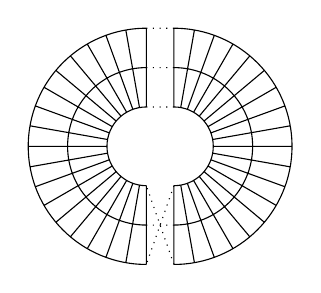
\begin{tikzpicture}[scale = 0.5]
        \begin{scope}[xshift = 0.35cm]
            \draw 
                (-90:1) arc (-90:90:1)
                (-90:2) arc (-90:90:2)
                (-90:3) arc (-90:90:3)
            \foreach\i in {-90,-80, ..., 90} {
                (\i:2) +(\i:-1) -- +(\i:1)
            };
        \end{scope}
        
        \begin{scope}[xshift = -0.35cm]
            \draw 
                (90:1) arc (90:270:1)
                (90:2) arc (90:270:2)
                (90:3) arc (90:270:3)
            \foreach\i in {90, 100, ..., 270} {
                (\i:2) +(\i:-1) -- +(\i:1)
            };
        \end{scope}
        \draw [dotted] 
            (0.35, 3) -- (-0.35, 3)
            (0.35, 2) -- (-0.35, 2)
            (0.35, 1) -- (-0.35, 1)
            (0.35, -1) -- (-0.35, -3)
            (0.35, -2) -- (-0.35, -2)
            (0.35, -3) -- (-0.35, -1)
            ;
    \end{tikzpicture}
    \caption{Das M\"obius-Band als nicht-triviales Vektorb\"undel \"uber der \(1\)-Sph\"are. Beachte, dass dieses nicht orientiert ist.}
\end{figure}

\section{Rahmungen}
    Um einen \(\mathbb{R}\)-Vektorr\"aum \(V\) effektiv betrachten zu k\"onnen, ist es stets n\"otig eine Basis \(\mathcal{B}\) zu w\"ahlen. Diese etabliert eine Vektorraumisomorphie \(\mathbb{R}^n\cong V\) und reduziert die Komplexit\"at der abstrakten Struktur von \(V\) auf den einfachst m\"oglichen Fall und etabliert einen \textit{Referenzrahmen}. Die Verallgemeinerung einer Basis auf Vektorr\"aume ist naheliegend, und besteht darin, dass auf stetige Art und Weise jeder Faser eine Basis zugeordnet wird. Hierbei existieren drei \"aquivalente Definitionen
\begin{definition}[Rahmen eines Vektorb\"undels]
    Sei \(\xi\colon E\to B\) ein Vektorb\"undel. Ein Rahmen ist 
    \begin{itemize}
        \item[i] eine Trivialisierung \(\xi\cong\underline{\mathbb{R}}^k\),
        \item[ii] die Wahl \(k\) linear unabh\"angiger Schnitte \(X_i\colon B\to E\) oder
        \item[iii] ein Schnitt im Rahmenb\"undel von \(\xi\).
    \end{itemize}
\end{definition}
Im Gegensatz zu Vektorr\"aumen, muss ein Rahmen keineswegs existieren. Viel eher ist die Existenz eines Rahmens eine starke Einschr\"ankung, da dies bereits impliziert, dass \(\xi\) trivial ist. Weiter sind unterschiedliche Rahmen nicht unbedingt zueinander \"aquivalent. Ein Vektorb\"undel zusammen mit einem Rahmen hei\ss e \textbf{gerahmtes Vektorb\"undel}. Die Wahl einer Rahmung von \(\xi\oplus\underline{\mathbb{R}}\) liefert eine \textbf{stabile Rahmung}. Wenn \(\xi\) zus\"atzlich orientierbar ist, ist es m\"oglich von orientierten Rahmungen zu sprechen. Im Folgenden seien alle Rahmungen orientiert. Seien \(F\) und \(G\) zwei Rahmungen eines Vektorb\"undels \(\xi\colon E\to B\). Dann sind sowohl \(F(p)\) als auch \(G(p)\) Basen von \(\xi^{-1}(p)\), und es kann der Basiswechsel \(M_{G(p)}^{F(p)}\in\operatorname{GL}^+(n)\) von \(F(p)\) zu \(G(p)\) betrachtet werden. Dies liefert eine stetige Funktion
\[M_G^F\colon B\to\operatorname{GL}^+(n),\,p\mapsto M_{G(p)}^{F(p)}\,,\]
den \textbf{Rahmenwechsel} von \(F\) zu \(G\). 
\begin{example}[Rahmenb\"undel der Sph\"are]\label{ex:framebundle_sphere}
    Der Tangentialvektorraum von \(\mathbb{S}^n\) an \(p\) kann als Untervektorraum des \(\mathbb{R}^{n+1}\) durch \(T_p\mathbb{S}^n\cong\{p\}^{\perp}\) identifiziert werden. Eine gegebene Orthonormalbasis \(b_i\) von \(T_p\mathbb{S}^n\subset\mathbb{R}^{n+1}\) kann also stets durch \(p\) zu einer Orthonormalbasis des \(\mathbb{R}^{n+1}\) erg\"anzt werden. Somit liegt die Matrix \(A:=(p,b_1,\dots,b_n)^{\intercal}\) in \(\operatorname{SO}(n+1)\) und es gilt \(A\cdot e_1=p\). Umgekehrt beschreibt eine Matrix \(B\in\operatorname{SO}(n+1)\) mit \(B\cdot e_1=p\) eine Orthonormalbasis von \(T_p\mathbb{S}^n\). Diese Korrespondenz liefert einen Hauptfaserb\"undelisomorphismus des orientiert orthonormalen Rahmenb\"undels der Sph\"are zu \(\operatorname{SO}(n+1)\). Weiter stiftet die Einh\"angung
    \[SA=\begin{pmatrix}
        A & 0\\
        0 & 1
    \end{pmatrix}\]
    eine Inklusion \(S\colon\operatorname{SO}(n)\hookrightarrow\operatorname{SO}(n+1)\) und f\"uhrt zu der im Folgenden au\ss erordentlich wichtigen Faserung
    \[\operatorname{SO}(n)\xrightarrow{S}\operatorname{SO}(n+1)\xrightarrow{\psi}\mathbb{S}^n\,.\]
    Eine tangentiale Rahmung der Sph\"are existiert nur f\"ur \(n\in\{1,3,7\}\), da nur in diesem Fall nullteilerfreie Multiplikationen auf dem \(\mathbb{R}^{n+1}\) existieren.
\end{example}

\subsection{Parallelisierbarkeit}
    Sei \(\mathcal{V}\) eine Mannigfaltigkeit. Dann sind das Tangentialb\"undel und gegebenenfalls auch das Normalenb\"undel definiert. Die Frage nach der Trivialit\"at dieser B\"undel erm\"oglicht einige Aussagen \"uber \(\mathcal{V}\) und m\"oglichweise den umliegenden Raum. \(\mathcal{V}\) hei\ss e (stabil) tangential oder normal gerahmt, wenn \(T\mathcal{V}\) oder \(N\mathcal{V}\) mit einer (stabilen) Rahmung versehen sind. Eine Mannigfaltigkeit mit stabil trivialem Tangentialb\"undel hei\ss e auch \textbf{\(\pi\)-Mannigfaltigkeit}. Die Signifikanz von \(\pi\)-Mannigfaltigkeiten der Dimension \(n\) f\"ur die Chirurgietheorie besteht darin, dass eingebettete \(k\)-Sph\"aren mit \(n\geq2k\) ein stabil triviales Normalenb\"undel besitzen, die Frage nach der eigentlichen Trivialit\"at etwas vereinfacht.

    \begin{theorem}\label{thm:vec_dim_triv}
        Sei \(\xi\) ein Vektorb\"undel vom Rang \(n\) \"uber einem \(k\)-dimensionalen CW-Komplex \(X\) mit \(n>k\). Dann ist \(\xi\) genau dann stabil trivial, wenn \(\xi\) bereits trivial ist.
    \end{theorem}
    \begin{proof}
        Sei \(F\colon\xi\oplus\underline{\mathbb{R}}\to\underline{\mathbb{R}}^{n+1}\) eine Trivialisierung. Diese liefert in jeder Faser eine Einbettung \(\xi^{-1}(p)\hookrightarrow\mathbb{R}^{n+1}\), sei etwa
        \[\xi^{-1}(p)\cong\{f(p)\}^{\perp}\cong T_{f(p)}\mathbb{S}^n\]
        f\"ur eine stetige Abbildung \(f\colon X\to\mathbb{S}^n\), die wegen \(n>k\) nullhomotop sein muss. Andererseits gilt nun \(\xi\cong f^*(T\mathbb{S}^n)\), sodass \(\xi\) bereits trivial sein muss.
    \end{proof}

    \begin{theorem}\label{thm:sub_pi_triv}
        Eine Untermannigfaltigkeit \(\mathcal{V}^k\) einer \(\pi\)-Mannigfaltigkeit \(\mathcal{M}^n\) mit \(n\geq2k\) ist genau dann eine \(\pi\)-Mannigfaltigkeit, wenn ihr Normalenb\"undel stabil trivial ist.
    \end{theorem}
    \begin{proof}
        Aus einer Zerlegung 
        \[T\mathcal{V}\oplus N\mathcal{V}\cong T\mathcal{M}|_{\mathcal{V}}\,,\]
        folgt
        \[T\mathcal{V}\oplus N\mathcal{V}\oplus\underline{\mathbb{R}}\cong T\mathcal{M}|_{\mathcal{V}}\oplus\underline{\mathbb{R}}\cong\underline{\mathbb{R}}^{n+1}\,.\]
        Somit ist einerseits \(T\mathcal{V}\oplus\underline{\mathbb{R}}^{n-k+1}\) trivial, wenn \(N\mathcal{V}\oplus\underline{\mathbb{R}}\) es ist, und andererseits \(N\mathcal{V}\oplus\underline{\mathbb{R}}^{k+1}\) trivial, wenn \(T\mathcal{V}\oplus\underline{\mathbb{R}}\) es ist. Aus Satz \ref{thm:vec_dim_triv} folgt, dass dann jeweils \(T\mathcal{V}\) und \(N\mathcal{V}\) stabil trivial sind.
    \end{proof}

    \begin{corollary}\label{cor:subsphere_stable}
        Jede in eine \(\pi\)-Mannigfaltigkeit eingebettete Sph\"are \(\mathcal{S}^k\hookrightarrow\mathcal{M}^n\) mit \(n\geq2k\) besitzt ein stabil triviales Normalenb\"undel.
    \end{corollary}
    \begin{proof}
        Das folgt aus Satz \ref{thm:sub_pi_triv}, da alle Sph\"aren \(\pi\)-Mannigfaltigkeiten sind \ref{cor:hom_pi}.
    \end{proof}
    

\section{Die Einh\"angung}
    Das Normalenb\"undel einer Mannigfaltigkeit \(\mathcal{M}^n\) ist stets von dem umliegenden Raum abh\"angig. Der Einbettungssatz von Whitney garantiert Einbettungen \(\mathcal{M}\hookrightarrow\mathbb{R}^m\) f\"ur \(m\geq2n\). F\"ur \(m\geq2n+2\) ist diese Einbettung bis aus Isotopie eindeutig bestimmt. Die Normalenb\"undel zweier solcher isotoper Einbettungen in einen \(\mathbb{R}^m\) sind isomorph, das Normalenb\"undel \textit{stabilisieriert} sich also. Dies motiviert den Begriff der Stabilisierung von Vektorb\"undeln.

\subsection{Die Einh\"angung}
    Sei \(f\in\operatorname{SO}(n)\). Dieses Element kann einerseits als stetige Abbildung
    \[f\colon\mathbb{S}^{n-1}\to\mathbb{S}^{n-1}\quad\text{mit}\quad Sf\colon S\mathbb{S}^{n-1}\to S\mathbb{S}^{n-1}\,,\]
    andererseits aber auch als lineare Abbildung
    \[f\colon\mathbb{R}^n\to\mathbb{R}^n\quad\text{mit}\quad Sf\colon\mathbb{R}^n\oplus\mathbb{R}\to\mathbb{R}^n\oplus\mathbb{R},\,x\mapsto\begin{pmatrix}
        A & 0\\
        0 & 1
    \end{pmatrix}\cdot x\,.\]
    verstanden werden. Jeweils ist \(Sf\in\operatorname{SO}(n+1)\) und definiert eine Inklusion \(S\colon\operatorname{SO}(n)\hookrightarrow\operatorname{SO}(n+1)\). Diese induziert offenbar einen Homomorphismus
    \[\pi_k(\operatorname{SO}(n))\xrightarrow{S_*}\pi_k(\operatorname{SO}(n+1))\,.\]
    Die gesamte Konstruktion erkl\"art einen Zusammenhang zwischen der topologischen Einh\"angung und der direkten Summe mit \(\mathbb{R}\). Zu einem orientierbaren Vektorb\"undel \(\xi\colon E\to\mathbb{S}^{k+1}\) mit Kupplungsfunktion \(\gamma\colon\mathbb{S}^k\to\operatorname{SO}(n)\) l\"asst sich diese Korrespondenz derart beschreiben, dass das Vektorb\"undel \(\xi\oplus\underline{\mathbb{R}}\to\mathbb{S}^{k+1}\), die Kupplungsfunktion \(S\gamma\) besitzt. 

\subsection{Die Stabilisierungsfolge der Sph\"are}\label{subsec:standard_frame_seq}
    Wie in Beispiel \ref{ex:framebundle_sphere} ist das Rahmenb\"undel der Sph\"are gerade \(\operatorname{SO}(n+1)\to\mathbb{S}^n\). Die Faser ist hierbei \(\operatorname{SO}(n)\). Dies liefert die wichtige Faserung
    \[\operatorname{SO}(n)\xrightarrow{S}\operatorname{SO}(n+1)\xrightarrow{\psi}\mathbb{S}^n\,,\]
    wobei \(S\) erneut die Einh\"angung bezeichne, und \(\psi(A)=A\cdot e_1\) sei. Zugeh\"orig zu jeder Faserung ist eine lange exakte Folge
    \[\pi_{k+1}\left(\mathbb{S}^n\right)\xrightarrow{\partial}\pi_k\left(\operatorname{SO}(n)\right)\xrightarrow{S_*}\pi_k\left(\operatorname{SO}(n+1)\right)\xrightarrow{\psi_*}\pi_k\left(\mathbb{S}^n\right)\xrightarrow{\partial}\pi_{k-1}\left(\operatorname{SO}(n)\right)\,.\]
    Diese ist besonders f\"ur \(k=n\) von Interesse. In diesem Fall wird der Generator \(\eqcl{\mathbbm{1}}\in\pi_n\left(\mathbb{S}^n\right)\) durch \(\partial\) auf die Kupplungsfunktion des Tangentialb\"undels abgebildet. Siehe auch \cite{knapp2013vektorbuendel} Korollar 3.3.4. Die Idee ist, dass sich die Identit\"at zu einer Funktion \(\mathbb{D}^n\to\operatorname{SO}(n+1)\) anheben l\"asst, die zu einer Rahmung des Tangentialb\"undels \"uber der oberen Hemisph\"are \(\mathbb{S}_+^n\cong\mathbb{D}^n\) homotop ist. Die Einschr\"ankung dieser Anhebung auf \(\mathbb{S}^{n-1}\) ist dann gerade der Rahmenwechsel dieser Rahmung zu der Standardrahmung der unteren Hemisph\"are. Ihre Homotopieklasse ist per Definition \(\eqcl{\tau_n}\). Der Kern \(\ker S_*\cong\im\partial\) wird also von \(\eqcl{\tau_n}\) erzeugt. 

\subsection{Normalenb\"undel eingebetteter Sph\"aren}\label{subsec:stable_normal_bundle}
    Sei \({n\geq2k}\), \(\mathcal{M}^n\) eine \(\pi\)-Mannigfaltigkeit und \({\mathcal{S}^k\hookrightarrow\mathcal{M}^n}\) eine eingebettete Sph\"a\-re, die gem\"a\ss{} Korollar \ref{cor:subsphere_stable} ein stabil triviales Normalenb\"undel \(\nu\) besitzt. Es gelten also 
    \[0=\eqcl{\nu\oplus\underline{\mathbb{R}}}=S_*\eqcl{\nu}\,\quad\text{beziehungsweise}\quad\eqcl{\nu}\in\ker S_*\,.\]
    Dann folgt aus dem Vorangegangenen, dass \(\eqcl{\nu}\) ein Vielfaches von \(\eqcl{\tau_k}\) ist. Weitere Kenntnisse \"uber den Rang von \(\eqcl{\tau_k}\) liefern
    \[\eqcl{\nu}\in\ker S_*\cong\begin{cases}
        \mathbb{Z} & k=2m\\
        \mathbb{Z}_2 & k=2m+1\notin\{1,3,7\}\\
        0 & k\in\{1,3,7\}
    \end{cases}\,.\]
    Siehe hierzu auch \cite{knapp2013vektorbuendel} Abschnitt 3.3.1.
    
\newpage
\section{Homotopiesph\"aren}
    Es ist nun naheliegend, die Menge \(\Theta_k\) mit der verbundenen Summe zu versehen. Es sind einige Lemmata notwendig, um zu zeigen, dass dies eine wohldefinierte Gruppenstruktur ergibt. 
\begin{lemma}\label{lem:simp_crit}
    Ein einfach zusammenh\"angender Kobordismus \(\mathcal{W}\) von \(\mathcal{M}\) zu \(\mathcal{N}\) ist genau dann ein H-Kobordismus, wenn \(H_*(\mathcal{W},\mathcal{M})=0\) gilt.
\end{lemma}
\begin{proof}
    Die Hinrichtung ist trivial. Seien nun \(H_*(\mathcal{W},\mathcal{M})=0\) und \(\iota\colon\mathcal{M}\hookrightarrow\mathcal{W}\) sowie \(j\colon\mathcal{N}\hookrightarrow\mathcal{W}\) die Inklusionen. Aus der Annahme folgt, dass  \(\iota\) ein Quasi-Isomorphismus ist. Dann folgt auch \(H^*(\mathcal{W},\mathcal{M})=0\) und aus der Lefschetz-Dualit\"at
    \[H_*(\mathcal{W},\mathcal{N})\cong H^{n+1-*}(\mathcal{W},\mathcal{M})=0\,,\]
    sodass auch \(j_*\) ein Quasi-Isomorphismus ist. Da \(\mathcal{W}\), \(\mathcal{M}\) und \(\mathcal{N}\) einfach zusammenh\"angend sind, folgt aus dem Satz von Whitehead, zusammen mit dem Satz von Hurewicz, dass die Inklusionen auch Homotopie\"aquivalenzen sind. 
\end{proof}
Das additive Inverse in \(\Theta_k\) ist offenbar die H-Kobordismus-Klasse der Standardsph\"are. Diese l\"asst sich wie folgt beschreiben.
\begin{lemma}\label{lem:h_cob_cont}
    Eine einfach zusammenh\"angende Mannigfaltigkeit \(\mathcal{M}^n\) ist genau dann Rand einer kontrahierbaren Mannigfaltigkeit \(\mathcal{W}^{n+1}\), wenn sie zu der Standardsph\"are H-kobordant ist.
\end{lemma}
\begin{proof}
    \subsubsection*{Hinrichtung}
        Sei \(\mathcal{M}\) Rand der kontrahierbaren Mannigfaltigkeit \(\mathcal{W}\). Sei \(\mathcal{D}\) eine eingebettete Scheibe und \({\mathcal{W}^{\prime}:=\mathcal{W}\setminus\mathring{\mathcal{D}}}\). Dann ist \(\partial\mathcal{W}^{\prime}\cong\mathcal{M}\sqcup-\mathcal{S}\) und \(\mathcal{W}^{\prime}\) ein Kobordismus. Per Ausschneidung folgt
        \[H_*(\mathcal{W}^{\prime},\partial\mathcal{D})\overcong{Aus.}H(\mathcal{W},\mathcal{D})\cong\Tilde{H}(\mathcal{W})=0\,,\]
        da \(\mathcal{W}\) einfach zusammenh\"angend ist, folgt aus Lemma \ref{lem:simp_crit}, dass \(\mathcal{W}^{\prime}\) ein H-Kobordismus ist.
        
    \subsubsection*{R\"uckrichtung}
        Sei \(\mathcal{M}\) mithilfe des Kobordismus \(\mathcal{W}^{\prime}\) zu der \(n\)-Sph\"are H-kobordant. Setze
        \[\mathcal{W}:=\mathcal{W}^{\prime}\mathop{+}^{\mathbb{S}^n}\mathbb{D}^{n+1}\,.\]
        Per Annahme gilt \(H_*(\mathcal{W}^{\prime},\mathbb{S}^n)=0\), sodass erneut
        \[H(\mathcal{W},\mathcal{D})\overcong{Aus.}H_*(\mathcal{W}^{\prime},\partial\mathcal{D})=0\]
        folgt. Da \(\mathcal{W}\) einfach zusammenh\"angend ist, ist sie zu dem kontrahierbaren Raum \(\mathcal{D}\) homotopie\"aquivalent und somit selbst kontrahierbar.
\end{proof}
\newpage
\begin{lemma}
    Das additive Inverse einer Homotopiesph\"are \(\mathcal{M}\) ist \(-\mathcal{M}\).
\end{lemma}
\begin{proof}
    W\"ahle eine Einbettung \(\Psi\colon\mathbb{R}^n+\mathbb{R}^n\hookrightarrow\mathbb{I}\times\mathbb{R}^n\) wie in Abbildung \ref{fig:sum_of_r}. F\"ur Details siehe \cite{kosinski1992differential} Kapitel VI Satz 1.3. Zu einer Verklebeabbildung \({\Phi\colon\mathbb{R}^n\hookrightarrow\mathcal{M}}\) ergibt dies eine Einbettung
    \[\im\Phi+\im\Phi\hookrightarrow\mathbb{I}\times\im\Phi\subseteq\mathbb{I}\times\mathcal{M}\,.\]
    Wird diese Einbettung \"uber \(\mathcal{M}\setminus\im\Phi\hookrightarrow0\times\mathcal{M}\) und \(-\mathcal{M}\setminus\im\Phi\hookrightarrow1\times\mathcal{M}\) zu einer Einbettung \(\mathcal{M}+(-\mathcal{M})\hookrightarrow\mathcal{M}\times\mathbb{I}\) fortgesetzt, ergibt sich eine Situation analog zu Abbildung \ref{fig:sum_of_r}. Das Bild dieser Einbettung, also auch \(\mathcal{M}+(-\mathcal{M})\), berandet eine Mannigfaltigkeit, die zu \(\mathcal{M}\), aus der eine offene Scheibe entfernt wurde, homotopie\"aquivalent ist. Diese muss jedoch kontrahierbar sein, da \(\mathcal{M}\) eine Homotopiesph\"are ist. Die Aussage folgt aus Lemma \ref{lem:h_cob_cont}.
\end{proof}

\begin{figure}
    \centering
    \begin{tikzpicture}
        \draw [pattern = north west lines]
            (-2.5, 1) -- node [above] {\(\mathbb{R}+\mathbb{R}\)} (-1.5, 1) arc (90:-90:1) -- (-2.5, -1);
        \draw [pattern = north west lines]
            (2.5, 1) -- (1.5, 1) arc (90:270:1) -- (2.5, -1)
            (-2.5, 0) edge [blue] (-0.5, 0) 
            (0.5, 0) edge [blue] (2.5, 0)
            (-3, 0) node {\(\mathbb{R}\setminus\mathring{\mathbb{D}}\)}
        ;
    \end{tikzpicture}
    \caption{Eine Einbettung \(\mathbb{R}+\mathbb{R}\hookrightarrow\mathbb{I}\times\mathbb{R}\). Ihr Bild berandet die schraffierte Mannigfaltigkeit, die die blaue Mannigfaltigkeit als Deformationsretrakt enth\"alt.}\label{fig:sum_of_r}
\end{figure}
\begin{lemma}
    Sind \(\mathcal{M}^n\) und \(\mathcal{M}^{\prime}\) geschlossen, einfach zusammenh\"angend und H-kobordant, sind es auch \(\mathcal{M}+\mathcal{N}\) und \(\mathcal{M}^{\prime}+\mathcal{N}\).
\end{lemma}
\begin{proof}
    Es kann angenommen werden, dass \(n\geq3\) ist. Sei \(\mathcal{W}_1\) ein H-Ko\-bor\-dis\-mus mit \(\partial\mathcal{W}_1=-\mathcal{M}^{\prime}\sqcup\mathcal{M}\). Da \(\mathcal{W}_1\) zu\-sam\-men\-h\"ang\-end ist, existiert eine Einbettung \(\iota\colon(\mathbb{I},\partial\,\mathbb{I})\hookrightarrow(\mathcal{W}_1,\partial\mathcal{W}_1)\) einer ordentlichen Untermannigfaltigkeit \(\mathcal{I}\), die Punkte \(p\in\mathcal{M}\) und \(p^{\prime}\in\mathcal{M}^{\prime}\) verbindet. Sei weiter \(\mathcal{W}_2:=\mathcal{N}\times\mathbb{I}\). Definiere den Kobordismus
    \[\mathcal{W}:=\mathcal{W}_1\mathop{+}^{\mathcal{I}}\mathcal{W}_2\quad\text{mit}\quad\partial\mathcal{W}\cong-\left(\mathcal{M}^{\prime}+\mathcal{N}\right)\sqcup\left(\mathcal{M}+\mathcal{N}\right)\,.\]
    Es bleibt zu zeigen, dass die Inklusionen \(\mathcal{M}+\mathcal{N}\hookrightarrow\mathcal{W}\) und \(\mathcal{M}^{\prime}+\mathcal{N}\hookrightarrow\mathcal{W}\) Homotopie\"aquivalenzen sind. Betrachte zun\"achst die Inklusion \(\iota\colon\mathcal{M}\hookrightarrow\mathcal{W}_1\). Da \(\mathcal{I}\cong\mathbb{I}\) kontrahierbar ist, ist das Normalenb\"undel in \(\mathcal{W}_1\) trivial, sodass eine Umgebung von \(\mathcal{I}\) zu \(\mathbb{I}\times\mathbb{R}^n\) diffeomorph ist. Das kommutative Diagramm
    \begin{equation}
        \begin{aligned}\label{eq:lem_sumHCob_01}
            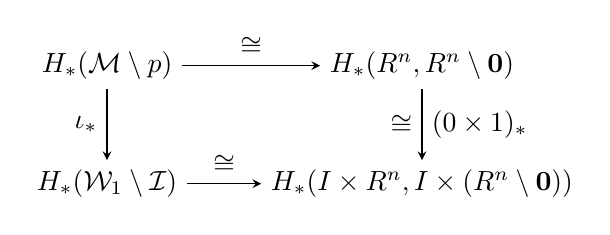
\begin{tikzpicture}
                \draw
                    (0, 0) node (A) {\(H_*(\mathcal{M}\setminus p)\)}
                    (4, 0) node (B) {\(H_*(\mathbb{R}^n,\mathbb{R}^n\setminus\mathbf{0})\)}
                    (0, -1.5) node (D) {\(H_*(\mathcal{W}_1\setminus\mathcal{I})\)}
                    (4, -1.5) node (E) {\(H_*(\mathbb{I}\times\mathbb{R}^n,\mathbb{I}\times(\mathbb{R}^n\setminus\mathbf{0}))\)}

                    (A) edge [-stealth] node [above] {\(\cong\)} (B)
                    (A) edge [-stealth] node [left] {\(\iota_*\)} (D)
                    (B) edge [-stealth] node [right] {\((0\times\mathbbm{1})_*\)} node [left] {\(\cong\)} (E)
                    (D) edge [-stealth] node [above] {\(\cong\)} (E)
                    ;
            \end{tikzpicture}
        \end{aligned}
    \end{equation}
    zeigt, dass die linke Abbildung ein Isomorphismus ist. Dann folgt aus dem F\"unfer\-lemma, dass auch die rechte Abbildung folgenden Diagrammes ein Isomorphismus sein muss.
    \begin{equation}
        \begin{aligned}\label{eq:lem_sumHCob_02}
            \begin{tikzpicture}
            \draw
                (0, 0) node (A) {\(H_*(\mathcal{M}\setminus p)\)}
                (3, 0) node (B) {\(H_*(\mathcal{M})\)}
                (6, 0) node (C) {\(H_*(\mathcal{M},\mathcal{M}\setminus p)\)}
                (0, -1.5) node (D) {\(H_*(\mathcal{W}_1\setminus\mathcal{I})\)}
                (3, -1.5) node (E) {\(H_*(\mathcal{W}_1)\)}
                (6, -1.5) node (F) {\(H_*(\mathcal{W}_1,\mathcal{W}_1\setminus\mathcal{I})\)}

                (A) edge [-stealth] (B)
                (A) edge [-stealth] node [left] {\(\cong\)} node [right] {\tiny\eqref{eq:lem_sumHCob_01}} (D)
                (B) edge [-stealth] (C)
                (B) edge [-stealth] node [left] {\(\cong\)} node [right] {\tiny H.Kob.} (E)
                (C) edge [-stealth] node [left] {\(\cong\)} node [right] {\tiny Fünferlemma} (F)
                (D) edge [-stealth] (E)
                (E) edge [-stealth] (F)
                ;
            \end{tikzpicture}
        \end{aligned}
    \end{equation}
    Betrachte nun die relative Mayer-Vietoris-Folge der Zerlegung von \((\mathcal{W},\mathcal{M}+\mathcal{N})\) durch die Bilder von \((\mathcal{W}_1\setminus\mathcal{I},\mathcal{M}\setminus p)\) und \((\mathcal{W}_2\setminus\mathbb{I},\mathcal{N}\setminus q)\). Es gilt
    \[H_*\left(\mathcal{W}_1\setminus\mathcal{I}\cap\mathcal{W}_2\setminus\mathbb{I},\mathcal{M}\setminus p\cap\mathcal{N}\setminus q\right)\cong H_*\left(\mathbb{I}\times(\mathbb{R}^n\setminus\mathbf{0}),\mathbb{R}^n\setminus\mathbf{0}\right)=0\,.\]
    Aus der Exaktheit der Mayer-Vietoris-Folge
    \[0\overeq{\eqref{eq:lem_sumHCob_02}}H_*(\mathcal{W}_1\setminus\mathcal{I},\mathcal{M}\setminus p)\oplus H_*(\mathcal{W}_2\setminus\mathbb{I},\mathcal{N}\setminus p)\to H_*(\mathcal{W},\mathcal{M}+\mathcal{N})\to0\,,\]
    folgt nun, dass auch \(H_*(\mathcal{W},\mathcal{M}+\mathcal{N})=0\) ist. Da \(\mathcal{W}\) f\"ur \(n\geq3\) weiterhin einfach zusammenh\"angend ist, folgt die Aussage aus Lemma \ref{lem:simp_crit}.
\end{proof}

\begin{lemma}
    Die verbundene Summe zweier Homotopiesph\"aren ist eine Homotopiesph\"are.
\end{lemma}
\begin{proof}
    F\"ur \(0<i<n\) gilt \(H_i(\mathcal{M}+\mathcal{N})\cong H_i(\mathcal{M})\oplus H_i(\mathcal{N})=0\), sodass \(\mathcal{M}+\mathcal{N}\) wegen
    \[H_0(\mathcal{M}+\mathcal{N})\cong H_n(\mathcal{M}+\mathcal{N})\cong\mathbb{Z}\quad\text{und}\quad H_j(\mathcal{M}+\mathcal{N})=0\quad\text{f\"ur}\quad j>n\]
    die gleichen Homologiegruppen wie die Sph\"are besitzt. Aus dem Satz von Seifert-van-Kampen folgt
    \[\pi_1(\mathcal{M}+\mathcal{N})\cong\pi_1(\mathcal{M})\times\pi_1(\mathcal{N})=0\]
    sodas \(\mathcal{M}+\mathcal{N}\) einfach zusammenh\"angend, und wegen dem Satz von Whitehead auch \((n-1)\)-zusammenh\"angend ist. Aus dem Satz von Hurewicz folgt, dass ein
    \[\eqcl{f}\in\pi_n(\mathcal{M}+\mathcal{N})\cong H_n(\mathcal{M}+\mathcal{N})\cong\mathbb{Z}\,,\]
    also eine Abbildung \(f\colon\mathbb{S}^n\to\mathcal{M}+\mathcal{N}\) des Grades eins existiert. Diese induziert in allen Dimensionen Isomorphismen \(f_*\colon H_i(\mathbb{S}^n)\to H_i(\mathcal{M}+\mathcal{N})\). Erneut folgt aus dem Satz von Whitehead, dass \(f\) eine Homotopie\"aquivalenz ist.
\end{proof}


\section{Die Thom-Pontrjagin-Konstruktion}
    Zwei geschlossene, normal gerahmte Untermannigfaltigkeiten \(\mathcal{M}^n\) und \(\mathcal{V}^n\) einer geschlossenen Mannigfaltigkeit \(\mathcal{N}^{n+k}\) hei\ss en gerahmt kobordant, falls ein Kobordismus \(\mathcal{W}^{n+1}\subseteq\mathcal{N}\times\mathbb{I}\) mit einer Rahmung existiere, die mit den Rahmungen von \(\mathcal{M}\) und \(\mathcal{V}\) \"ubereinstimmt. Die Menge der \"Aquivalenzklassen zusammen mit der disunkten Vereinigung bildet f\"ur \(k\geq n+2\) eine abelsche Gruppe \cite{kosinski1992differential} Kapitel IX Satz 3.1. Das Nullelement ist hierbei trivialerweise die \"Aquivalenzklasse der leeren Mannigfaltigkeit. Ein Repr\"asentant dessen ist durch die Standardsph\"are mit der \textit{Standard-Rahmung} gegeben. Diese ist durch kanonische Identifizierungen des nach au\ss en  gerichtete Normalenvektors \(n(p)\in N_p\mathbb{S}^n\subseteq\mathbb{R}^{n+k}\) zusammen mit den Vektoren \(e_{n+2},\dots,e_{n+k}\) gegeben. Inverse Elemente sind \"Aquivalenzklassen der gleichen Mannigfaltigkeit, in welchem ein Basisvektor \(v\) mit \(-v\) ersetzt wurde. Die derartig erhaltene Gruppe sei durch \(\Omega_n^{\text{\tiny Fr}}(\mathcal{N})\) bezeichnet.
\begin{figure}
    \centering
    \tdplotsetmaincoords{60}{110}
    \tdplotsetthetaplanecoords{0}
    
    \begin{tikzpicture}[scale = 2.5, tdplot_main_coords]
        \draw[dashed,tdplot_rotated_coords] (0,-1,0) arc (-90:90:1);
        \draw[tdplot_rotated_coords]
        \foreach \i in {-60, -30,..., 60} {
            (\i:1) ++(\i:0.25) edge[stealth-] (\i:1)
        };
        \draw
        \foreach \i in {0,45, ..., 360} {
            (\i:1) ++(\i:0.25) edge[stealth-] (\i:1)
        }
        \foreach \i in {45, 135} {
            (\i:1cm and 1cm) ++(\i:0.25cm and 0.25cm) edge[stealth-] (\i:1cm and 1cm)
        };
        \draw [dashed] (180:1cm and 5mm) arc (180:0:1cm and 1cm) (1, 0, 0) arc (0:360:1);
        \shade[ball color=blue!10!white,opacity=0.2] (1cm, 0) arc (0:-180:1cm and 5mm) arc (180:0:1cm and 1cm);
    \end{tikzpicture}
    \caption{Die Standardrahmung von \(\mathbb{S}^1\subset\mathbb{R}^2\), und der gerahmte Nullbordismus \(\mathbb{S}_+^2\subset\mathbb{R}^3\).}
\end{figure}

\subsection{Thom-Pontrjagin-Kollapsabbildungen}
    Nach dem Satz von Sard besitzt jede Funktion \(f\colon\mathcal{N}^{n+k}\to\mathbb{S}^k\) einen regul\"aren Wert \(\star\in\mathbb{S}^k\), wobei das Urbild eines regul\"aren Wertes stets eine \(n\)-dimensionale Untermannigfaltigkeit \(f^{-1}(\star)\subseteq\mathcal{N}\) ergibt. Da \(\star\) eine nulldimensionale Mannigfaltigkeit ist, besitzt diese ein triviales Normalenb\"undel. Eine Rahmung dieser (also eine Wahl einer positiv orientierten Basis \(\phi\) von \(T_{\star}\mathbb{S}^k\)) l\"asst sich zu einer normalen Rahmung von \(f^{-1}(\star)\) zur\"uckziehen. Unterschiedliche regul\"are Punkte oder unterschiedliche positiv orientierte Basen ergeben hierbei zueinander gerahmt kobordante Mannigfaltigkeiten. Folglich l\"asst sich die Abbildung
    \[\Tilde{p}\colon\mathcal{C}^{\infty}(\mathcal{N},\mathbb{S}^k)\to\Omega_n^{\text{\tiny Fr}}(\mathcal{N}),\,f\mapsto\eqcl{\left(f^{-1}(\star),(\dx f)^*(\phi)\right)}\]
    definieren. Eine glatte Homotopie \(H\colon\mathcal{N}\times\mathbb{I}\to\mathbb{S}^k\) mit regul\"arem Punkt \(\star\) zwischen zwei Abbildungen \(f,g\in\mathcal{C}^{\infty}(\mathcal{N},\mathbb{S}^k)\) birgt nun den gerahmten Kobordismus \(H^{-1}(\star)\subseteq\mathcal{N}\times\mathbb{I}\) zwischen \(f^{-1}(\star)\) und \(g^{-1}(\star)\). Auf diese Art und Weise induziert \(\tilde{p}\) eine Abbildung \(p\colon\eqcl{\mathcal{N},\mathbb{S}^k}\to\Omega_n^{\text{\tiny Fr}}(\mathcal{N})\). Umgekehrt l\"asst sich einer Mannigfaltigkeit \(\mathcal{M}^n\subseteq\mathcal{N}^{n+k}\) mit einer  Trivialisierung \(\Phi\colon N\mathcal{M}\to\mathcal{M}\times\mathbb{R}^k\) folgenderma\ss en eine Funktion \(f\colon\mathcal{N}\to\mathbb{S}^k\) mit \(\mathcal{M}=f^{-1}(\star)\) zuordnen. Sei \(\Psi\colon N\mathcal{M}\hookrightarrow\mathcal{N}\) eine Tubenumgebung mit Bild \(U\subseteq\mathcal{N}\). Dann kann gem\"a\ss{} Diagramm \ref{dia:gen_map} eine glatte Abbildung \(f\colon U\to\mathbb{S}^k\setminus\{-\star\}\) konstruiert werden, die durch
    \[\Tilde{f}\colon\mathcal{N}\to\mathbb{S}^k,\,x\mapsto\begin{cases}
        f(x) & x\in U\\
        -\star & \text{sonst}
    \end{cases}\]
    auf \(\mathcal{N}\) fortgesetzt werden kann, \(\Tilde{f}^{-1}(\star)=\mathcal{M}\) erf\"ullt, und die Rahmung \(\Phi\) induziert. Bei der Konstruktion sei beachtet, dass sich unterschiedliche Basen von \(T_{\star}\mathbb{S}^n\) bez\"uglich einer Funktion zwar zu \"aquivalenten Rahmungen zur\"uckziehen, dass eine Mannigfaltigkeit zu unterschiedlichen Rahmungen jedoch sehr wohl in unterschiedlichen gerahmten Kobordanzklassen liegen kann. Von besonderem Interesse ist der Fall \({\mathcal{N}=\mathbb{S}^{n+k}}\), da \(\eqcl{\mathbb{S}^{n+k},\mathbb{S}^k}=\pi_{n+k}(\mathbb{S}^k)\) ist. Siehe f\"ur weitere Informationen \cite{milnor1965topology} \S7.

    \begin{figure}
        \centering
        \begin{tikzpicture}
            \draw   node (A) {\(U\subseteq\mathcal{N}\)}
                    node [above = of A] (B) {\(N\mathcal{M}\)}
                    node [right = of B] (C) {\(\underline{\mathbb{R}}^k\)}
                    node [right = of C] (D) {\(\mathbb{R}^k\)}
                    node [below = of D] (E) {\(\mathbb{S}^k\setminus\{-\star\}\)}
                    (B) edge [bend right = 35, ->] node [sloped, above, rotate = 180] {\(\cong\)} node [left] {\(\Psi\)} (A)
                    (B) edge [bend left = 35, ->] node [below] {\(\cong\)} node [above] {\(\Phi\)} (C)
                    (A) edge [bend right = 35, ->] node [sloped, above] {\(\cong\)} (C)
                    (C) edge [bend left = 35, ->] node [above] {\(\pi_2\)} (D)
                    (D) edge [bend left = 35, ->] node [sloped, above] {\(\cong\)} (E)
                    (A) edge [bend right = 25, ->] node [sloped, above] {\(f\)} (E);
        \end{tikzpicture}
        \caption{Die Konstruktion einer \(\mathcal{M}\) generierenden Abbildung \(f\).}
        \label{dia:gen_map}
    \end{figure}

    \begin{proposition}[Thom-Pontrjagin]
        Die Gruppen \(\Omega_n^{\textup{\tiny Fr}}(\mathbb{S}^{n+k})\) und \(\pi_{n+k}(\mathbb{S}^{k})\) sind isomorph.
    \end{proposition}
    \noindent Insbesondere wird die Folge der \(\pi_{n+k}(\mathbb{S}^k)\), also auch die Folge der \(\Omega_n^{\text{\tiny Fr}}(\mathbb{S}^{n+k})\) f\"ur \(k\geq n+2\) station\"ar. Setze
    \[\Omega_n^{\text{\tiny Fr}}:=\lim_{k\to\infty}\Omega_n^{\textup{\tiny Fr}}(\mathbb{S}^{n+k})\cong\lim_{k\to\infty}\pi_{n+k}(\mathbb{S}^k)=\Pi_n\,.\]
    Es stellt sich in der obigen Definition die Frage, warum die disjunkte Summe anstatt der verbundenen Summe als Gruppenoperation gew\"ahlt wird. Die Antwort darauf liegt in dem durch die verbundene Randsumme erhaltenen Kobordismus
    \[\mathcal{W}=\mathcal{M}\times\mathbb{I}+\mathcal{N}\times\mathbb{I}\quad\text{mit}\quad\partial\mathcal{W}\cong(-\mathcal{M})\sqcup(-\mathcal{N})\sqcup(\mathcal{M}+\mathcal{N})\,.\]
    Gegebene Rahmungen \(F\) und \(G\) von \(\mathcal{M}\) und \(\mathcal{N}\) induzieren eine Rahmung auf \(\mathcal{W}\) und damit auf \(\mathcal{M}+\mathcal{N}\). Folglich sind \({(\mathcal{M},F)\sqcup(\mathcal{N},G)}\) und \({(\mathcal{M}+\mathcal{N},H)}\) gerahmt kobordant, sodass die disjunkte Summe und die verbundene Summe tats\"achlich die gleiche Gruppenoperation bestimmen.


\section{Der \texorpdfstring{\(J\)}{TEXT}-Homomorphismus}
    Sei \(\gamma\colon\mathbb{S}^n\to\operatorname{SO}(k)\) glatt und \((\mathbb{S}^n,E)\) die Standardsph\"are mit der Standardrahmung des Normalenb\"undels im \(\mathbb{R}^{n+k}\). Dann existiert genau eine normale Rahmung \(\Gamma\) von \(\mathbb{S}^n\), sodass der Rahmenwechsel von \(E\) zu \(\Gamma\) gerade \(\gamma\) ist. F\"ur \(\Gamma\) kann also
\[\Gamma_i(p)=\sum_{j=1}^k\gamma_{ij}(p)E_j(p)\]
als Definition genutzt werden. Dies liefert die normal gerahmte Mannigfaltigkeit \((\mathbb{S}^n,\Gamma)\in\Omega_n^{\text{\tiny Fr}}(\mathbb{S}^{n+k})\) und (auch wenn noch nicht klar ist dass diese wohldefiniert ist) eine Abbildung
\[J_n^k\colon\pi_n(\operatorname{SO}(k))\to\Omega_n^{\text{\tiny Fr}}(\mathbb{S}^{n+k})\,.\]
Sei nun \(\eqcl{\gamma}\in\ker J_n^k\), es gelte also \(J_n^k\eqcl{\gamma}=0\). Dann ist \((\mathbb{S}^n,\Gamma)\) gerahmt nullbordant. Das ist genau dann der Fall, wenn sich \(\Gamma\) auf eine Mannigfaltigkeit \(\mathcal{M}^{n+1}\subseteq\mathbb{R}_+^{n+k+1}\) mit \(\partial\mathcal{M}\cong\mathbb{S}^n\) fortsetzen l\"asst. F\"ur hinreichend gro\ss es \(k\), also f\"ur \(k\geq n+2\), stabilisiert sich diese Definition, und es ergibt sich der \textbf{Hopf-Whitehead-J-Homomorphismus}
\[J_n\colon\pi_n(\operatorname{SO})\to\Pi_n\,.\]
\begin{proposition}\label{prop:adams_order}
    Das Bild \({\im J_{4m-1}}\) ist eine zyklische Gruppe des Ranges
    \[\operatorname{Rang}\operatorname{Im}J_{4m-1}=\operatorname{Nenner}\left(\frac{B_{2m}}{4m}\right)\]
    und ein direkter Summand von \(\Pi_{4m-1}\).
\end{proposition}
\begin{proof}
    Siehe \cite{adams1966groups} Satz 1.5.
\end{proof}